\begin{figure}[H]
    \subfloat[Didascalia immagine 1]{
        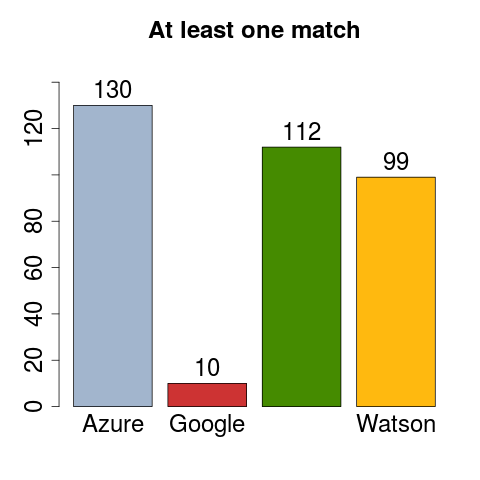
\includegraphics[width=0.45\linewidth]
        {immagine1}
    }
    \hfill
    \subfloat[Didascalia immagine 2]{
        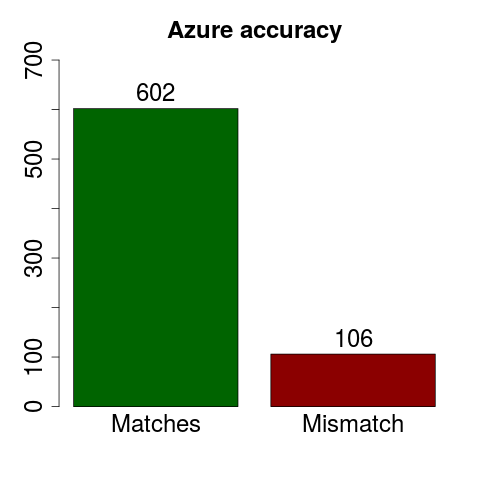
\includegraphics[width=0.45\linewidth]
        {immagine2}
    }
    \\
    \subfloat[Didascalia immagine 3]{
        
\includegraphics[width=\linewidth]
        {immagine3}
    }
    \\
    \subfloat[Didascalia immagine 4]{
        
\includegraphics[width=0.60\linewidth]
        {immagine4}
    }
    \caption{Didascalia globale delle 4 immagini}
\end{figure}